\subsection{General Results on Groups}

\begin{lemma}
    \label[lemma]{lem:grouprop}
    Suppose \(G\) is a group. Then
    \begin{enumerate}[(1)]
        \item The identity is unique
        \item Inverses are unique
        \item For every \(a,b,c\in G\) there is a unique \(x \in G\) s.t. \(ax=b\)
        \item If \(ab=ac\) then \(b=c\), similarly if \(xy=zy\) then \(x=z\)
        \item \((ab)^{-1}=b^{-1}a^{-1}\)
        \item If \((ab)^2=a^2b^2\) then \(ab=ba\)
        \item If \(\t{ord}(g)=2\) for all \(g \in G\) then \(G\) is abelian
    \end{enumerate}
\end{lemma}

\begin{itemize}
    \item \begin{proof}(3)
        Let \(ax=b\implies x=a^{-1}b\)
    
        Suppose \(x,y\in G \t{ s.t.} ax=b \t{ and } ay=b\)
    
        \(ax=ay\implies x=y\)
    \end{proof}
    \item \begin{proof}(6)
        Assume \((ab)^2=a^2b^2\)

       \(ab=(a^{-1}a)(ab)(bb^{-1})=a^{-1}a^2b^2b^{-1}=a^{-1}(ab)^2b^{-1}=(a^{-1}a)(ba)(bb^{-1})=ba\)
    \end{proof}
    \item \begin{proof}
        Assume \(\t{ord}(g)=2\) for all \(g \in G\)

        \(\implies g=g^{-1}\) for all \(g \in G\)

        Let \(a,b \in G\). Consider \(ab\)

        \(ab=(ab)^{-1}=b^{-1}a^{-1}=ba\)
    \end{proof}
\end{itemize}

\begin{definition}\label[definition]{def:subgroup}
    Given a group \(G\) and a subset \(H\subseteq G\), we say \(H\) is a subgroup
    \(H \leq G\) if 
    \begin{itemize}
        \item The identity of \(G\) is in \(H\)
        \item For all \(h \in H, h^{-1}\in H\)
        \item For all \(a,b\in H\), \(ab\in H\)
    \end{itemize}
\end{definition}

\begin{theorem}
    \label[theorem]{thm:subgrouptest}
    Suppose that \(G\) is a group and \(\emptyset\neq H \subseteq G\)
    \\then \(H \leq G \iff\) for all  \(a,b \in H, ab^{-1}\in H\)
\end{theorem}

\begin{proof}
    \phantom{t}

    (\(\implies\)) Assume \(H \leq G\)

    Let \(a,b\in H\)

    By \Cref{def:subgroup} \(\implies b^{-1}\in H \implies ab^{-1} \in H\)
    \\\phantom{text}

    (\(\Longleftarrow\)) Assume for all \(a,b \in H\), \(ab^{-1}\in H\)

    \begin{itemize}
        \item (Identity) Consider \(a\in H\)
        
        \(\implies aa^{-1}=e\in H\)

        \item (Inverses) \checkmark
        \item (Closure) Consider \(a,b^{-1}\in H\)
        
        \(\implies ab \in H\)
    \end{itemize}
\end{proof}

\subsubsection{Subgroup Lattice}
\paragraph*{Subgroup of Order 4}
\begin{center}
    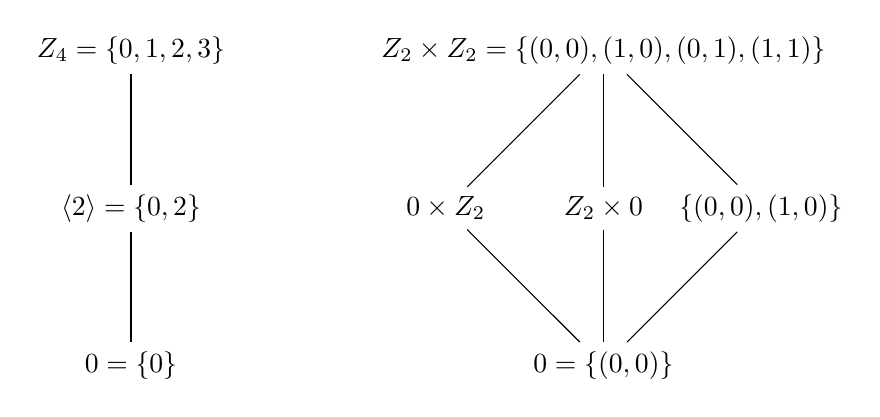
\begin{tikzpicture}
        % Define the nodes
        \node (Z4) at (-3,4) {$\mathbb{Z}_4 = \{0,1,2,3\}$};
        \node (gen2) at (-3,2) {$\langle 2 \rangle = \{0,2\}$};
        \node (zero) at (-3,0) {$0 = \{0\}$};
        
        \node (Z2x0) at (3,2) {$\mathbb{Z}_2 \times 0$};
        \node (0xZ2) at (1,2) {$0 \times \mathbb{Z}_2$};
        \node (Z2xZ2) at (3,4) {$\mathbb{Z}_2 \times \mathbb{Z}_2 = \{(0,0),(1,0),(0,1),(1,1)\}$};
        \node (0x11) at (5,2) {$\{(0,0),(1,0)\}$};
        \node (zero2) at (3,0) {$0 = \{(0,0)\}$};

        % Draw the lines
        \draw (Z4) -- (gen2);
        \draw (gen2) -- (zero);
        \draw (Z2xZ2) -- (Z2x0);
        \draw (Z2xZ2) -- (0xZ2);
        \draw (Z2xZ2) -- (0x11);
        \draw (Z2x0) -- (zero2);
        \draw (0xZ2) -- (zero2);
        \draw(0x11) -- (zero2);
    \end{tikzpicture}
\end{center}
\newpage
\paragraph*{Subgroup of Order 6}
\begin{center}
    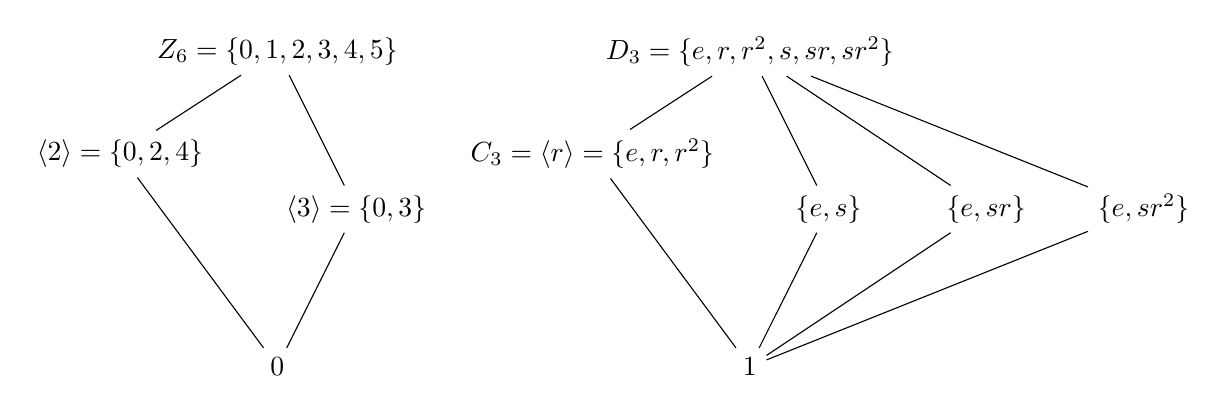
\begin{tikzpicture}
        % Define the nodes
        \node (Z6) at (-3,4) {$\mathbb{Z}_6 = \{0,1,2,3,4,5\}$};
        \node (gen2) at (-5,2.7) {$\langle 2 \rangle = \{0,2,4\}$};
        \node (gen3) at (-2,2) {$\langle 3 \rangle = \{0,3\}$};
        \node (zero) at (-3,0) {$0$};
    
        \node (D3) at (3,4) {$D_3 = \{e,r,r^2,s,sr,sr^2\}$};  
        \node (genr) at (1,2.7) {$C_3=\langle r \rangle = \{e,r,r^2\}$};
        \node (s) at (4,2) {$\{e,s\}$};
        \node (sr) at (6,2) {$\{e,sr\}$};
        \node (sr2) at (8,2) {$\{e,sr^2\}$};
        \node (1) at (3,0) {$1$};

        % Draw the lines
        \draw (Z6) -- (gen2) -- (zero);
        \draw (Z6) -- (gen3) -- (zero);

        \draw (D3) -- (genr) -- (1);
        \draw (D3) -- (s) -- (1);
        \draw (D3) -- (sr) -- (1);
        \draw (D3) -- (sr2) -- (1);
    \end{tikzpicture}
\end{center}

\begin{definition}
    Given a group \(G\) and a subset \(S \subseteq G\)
    \begin{itemize}
        \item The centralizer of \(S\) in $G$: \(C_G(S)=\left\{ g \in G \mid gs=sg,\;\; \forall s\in S \right\}\)
        \item The center of $G$: \((C_G(G)) = Z(G)=\left\{ z \in G \mid gz=zg,\;\; \forall g\in G \right\}\) 
    \end{itemize}
\end{definition}

\begin{lemma}\label[lemma]{lem:centersubgroup}
    \(C_G(S) \t{ and } Z(G)\) are subgroups of $G$
\end{lemma}
\begin{proof}
    Both contain $e$ so they are nonempty

    Let \(a,b \in C_G(S)\) and \(s \in S\)

    Consider:

    \begin{align*}
        as&=sa\\
        sab^{-1}&=asb^{-1}\\
                &=a(b^{-1}b)sb^{-1}\\
                &=(ab^{-1})s
    \end{align*}

    Thus $ab^{-1} \in S$

    Thus, by \Cref{thm:subgrouptest} $C_G(S)$ is a subgroup

    \(\implies Z(G) \leq G\) since the center is a special case of the centralizer
\end{proof}
\newpage
\begin{example}
    Centralizers in $D_4$

    \begin{itemize}
        \item $C_{D_4}(e)=D_4=C_{D_4}(r^2)\;\;$\footnote{Since $r^2s=sr^2$ and $r^2r=rr^2$}
        \item $C_{D_4}(r)={e,r,r^2,r^3}=C_{D_4}(r^3)$
        \item $C_{D_4}(s)={e,s,r^2,sr^2}=C_{D_4}(sr^2)$
        \item $C_{D_4}(sr)={e,sr,r^2,sr^3}=C_{D_4}(sr^3)$
        \item $Z(D_4)={e,r^2}$
    \end{itemize}
\end{example}